\documentclass[cn]{elegantbook}

\usepackage[all]{xy}
\usepackage{amsmath}
\usepackage{asymptote}

\newcount\mycount
%\def\ConvColor{rgb:yellow,5;red,2.5;white,5}
%\def\ConvReluColor{rgb:yellow,5;red,5;white,5}
%\def\PoolColor{rgb:red,1;black,0.3}
%\def\FcColor{rgb:blue,5;red,2.5;white,5}
%\def\FcReluColor{rgb:blue,5;red,5;white,4}
%\def\SoftmaxColor{rgb:magenta,5;black,7}

% title info
\title{数学女孩}
\subtitle{读书笔记}

% bio info
\author{虞朝阳}
\institute{西北工业大学}
%\date{\today}

% extra info
\version{1.00}
\equote{Wir m\"ussen wissen, wir werden wissen. (我们必须知道,我们必将知道) - David.Hilbert}
%\logo{logo.png}
\cover{cover.jpg}

\begin{document}

\maketitle

\chapter*{前言}
\addcontentsline{toc}{chapter}{Preface}
\markboth{Preface}{}
这里把《数学女孩》I\cite{mathgirl2016}中的一些问题收集整理到一起。


\tableofcontents
\mainmatter
\hypersetup{pageanchor=true}

% add preface chapter here if needed
\chapter{质因数之和}
首先看一个具体的例子,看看1024的所有约数的和。1024的所有约数是
\[
2^0, 2^1, 2^2, 2^3, 2^4, 2^5, 2^6, 2^7,2^8, 2^9, 2^{10},
\]
这些约数的和
\[
2^0 + 2^1 + 2^2 + 2^3 + 2^4 + 2^5 + 2^6 + 2^7 + 2^8 + 2^9 + 2^{10} = 2^{11}-1.
\]
$n=p^m$的情形,这里$p$为素数,$p^m$的所有约数之和为
\[
p^0 + p^1 + \cdots + p^m = \frac{1-p^{m+1}}{1 - p}.
\]
对于一般情形,将正整数$n$进行素因数分解,
\[
n = p_0^{a_0} \times p_1^{a_1} \times \cdots \times p_m^{a_m},
\]
$n$的约数具有形式
\[
p_0^{b_0} \times p_1^{b_1} \times \cdots \times p_m^{b_m},
\]
其中$b_k$从$0$到$a_k$。所有的约数的和是:
\[
\begin{aligned}
\varphi(n) &= (1 + p_0 + p_0^2 + \cdots + p_0^{a_0}) \\
& \times (1 + p_1 + p_1^2 + \cdots + p_1^{a_1}) \\
& \times \cdots \\
& \times (1 + p_m + p_m^2 + \cdots + p_m^{a_m}) \\
&= \frac{1-p_0^{a_0+1}}{1-p_0}\cdot\frac{1-p_1^{a_1+1}}{1-p_1}\cdots\frac{1-p_m^{a_m+1}}{1-p_m} \\
&= \prod_{k=0}^{m}{\frac{1-p_k^{a_k+1}}{1-p_k}}.
\end{aligned}
\]
使用符号,这样来理解,
\[
\begin{aligned}
&\sum_{b_0=0}^{a_0}\cdots\sum_{b_m=0}^{a_m}{p_0^{b_0} \times \cdots \times p_m^{b_m}} \\
=&\sum_{b_0=0}^{a_0}{p_0^{b_0}} \times \cdots \times \sum_{b_m=0}^{a_m}{p_m^{b_m}}.
\end{aligned}
\]
这个乘积的形式可以和组合联系起来,在$m$个组成各个因子的和式中,从中各自选择一个$p_k^{b_k}$就可以组合得到$n$的一个约数.

\chapter{复数}
复数$x+iy$可以和点$(x,y)$相联系,也可以和矩阵
\[
\begin{pmatrix} \cos{\theta} & -\sin{\theta} \\ \sin{\theta} & \cos{\theta} \end{pmatrix}
\]
相联系,与矩阵联系的是复数$\cos\theta + i\sin\theta$.从几何上讲,复数的相乘,矩阵相乘都可以和旋转相联系.这里我们有棣莫弗公式:
\[
(\cos\theta + i\sin\theta)^n =\cos n\theta + \sin n\theta.
\]
说明$n$次旋转角度$\theta$,等于一次旋转角度$n\theta$.由此可以推导三角函数中的各种倍角公式之类的.

\chapter{斐波那契数列和生成函数}
我们把一个数列和无穷级数对应起来,如下图所示:
\[
\begin{aligned}
\text{数列}\quad & \longleftrightarrow && \text{函数} \\
(a_0, a_1, \cdots, a_n, \cdots) \quad & \longleftrightarrow && a_0 + a_1x + \cdots + a_nx^n+\cdots
\end{aligned}
\]
这个无穷级数就称为生成函数。这一节的目的是通过生成函数来求出数列的通项公式。通过生成函数把数列中的各项作为整体进行考虑,可以把离散问题,转化为连续问题,使用微积分中的一些方法。
\[
\begin{array}{ccc}
\text{数列} & \longrightarrow & \text{生成函数} \\
&& \downarrow \\
\text{数列的通项} &\longleftarrow & \text{生成函数的有限项代数式} \\
\end{array}
\]

对于斐波那契数列($0,1,1,2,3,5,8,\cdots$)有如下递推公式:
\[
F_n = \left\{
\begin{aligned}
&0 &&(n=0)\\
&1 &&(n=1)\\
&F_{n-2} + F_{n-1}&&(n \ge 2)
\end{aligned}\right.
\]
对应的生成函数
\[
\begin{aligned}
F(x) &= F_0x^0 + F_1x^1 + F_2x^2 + F_3x^3 + \cdots + F_nx^n + \cdots\\
&= 0x^0 + 1x^1 + 1x^2 + 2x^3 + \cdots \\
&= x + x^2 + 2x^3 + \cdots
\end{aligned}
\]
接下来需要找出$F(x)$的有限项代数式,这里需要使用$F_n$的递推式。只需要如下所示:
\[
\begin{aligned}
A:\quad &F(x) \cdot x^2 &=& &&F_0x^2 + F_1x^3 + F_2x^4+\cdots \\
B:\quad &F(x) \cdot x^1 &=& &F_0x^1 + &F_1x^2 + F_2x^3+F_3x^4+\cdots \\
C:\quad &F(x) \cdot x^0 &=& F_0x^0 + &F_1x^1 + &F_2x^2+F_3x^3+F_4x^4+\cdots
\end{aligned}
\]
于是我们看看$A+B-C$得到什么。左边变为
\[
F(x)\cdot(x^2 + x^1-x^0) = F(x)(x^2+x-1)
\]
右边是
\[
\begin{aligned}
&F_0x^1 - F_0x^0 - F_1x^1 \\
&+(F_0 + F_1 - F_2) \cdot x^2 \\
&+(F_1 + F_2 - F_3) \cdot x^3 \\
&+(F_2 + F_3 - F_4) \cdot x^4 \\
&+ \cdots \\
&+(F_{n-2} + F_{n-1} - F_n) \cdot x^n \\
&+ \cdots \\
&=-x
\end{aligned}
\]
于是我们得到
\[
F(x) \cdot(x^2+x-1) = -x,
\]
进一步得到$F(x)$的有限项代数式:
\[
F(x) = \frac{x}{1-x-x^2},
\]
接下来需要重新把这个$F(x)$的有限项代数式表示为无穷级数,对于这个有理分式,相对简单,如果是其他的,应该借助于泰勒展开式。

对于有理分式,在复数范围内,最终可以分解为如下形式的和
\[
\frac{1}{x+a},
\]
而在实数范围,可以表示成如下两种形式的分式之和:
\[
\frac{1}{x+a}, \quad \frac{a+bx}{x^2+cx+d},
\]
对于
\[
\frac{1}{x+a},
\]
可以通过提取一个常数,最终转化为形式
\[
\frac{1}{1-ax},
\]
注意到等比级数的和的公式,我们有
\[
\frac{1}{1-ax} = \sum_{n=0}^{+\infty}{a^nx^n}.
\]
所以对于斐波那契数列的生成函数$F(x)$只需进行有理分式的分解即可,分解方法使用待定系数法。
\[
\begin{aligned}
\frac{x}{1-x-x^2} &= \frac{R}{1-rx} + \frac{S}{1-sx} \\
&=\frac{(R+S) - (rS + sR)x}{1 - (r+s)x + rsx^2}.
\end{aligned}
\]
由此可得4个未知数4个独立等式的方程组,
\[
\left\{
\begin{aligned}
R+S &= 0\\
rS+sR&= -1 \\
r+s &=1\\
rs&= -1
\end{aligned}
\right.
\]
解出这4个未知数,然后利用等比级数,最终可以得到斐波那契数列的通项公式
\[
F_n = \frac{1}{\sqrt{5}}((\frac{1 + \sqrt{5}}{2})^n - (\frac{1 - \sqrt{5}}{2})^n)
\]

\chapter{微分和差分}
微分对应的是连续函数,差分对应的就是离散函数,我们需要经常在两个世界进行转换。为了方便,首先定义一个符号,下降阶乘幂:
\[
x^{\underline{n}} = (x-0)(x-1)\cdots(x-(n-1)),
\]
这里的n是正整数,那么对于n为负整数的时候,如何定义呢?通过如下方式类推:
\begin{itemize}
\item 将$x^{\underline{3}}$除以$(x-2)$得到$x^{\underline{2}}$,
\item 将$x^{\underline{2}}$除以$(x-1)$得到$x^{\underline{1}}$,
\end{itemize}
那么后面应该是
\begin{itemize}
\item 将$x^{\underline{1}}$除以$(x-0)$得到$x^{\underline{0}}$,
\item 将$x^{\underline{0}}$除以$(x+1)$得到$x^{\underline{-1}}$,
\item 将$x^{\underline{-1}}$除以$(x+2)$得到$x^{\underline{-2}}$,
\end{itemize}
于是我们又有这个针对所有整数的下降阶乘幂的定义
\[
x^{\underline{n}} = \left\{
\begin{aligned}
&(x-0)(x-1)\cdots(x-(n-1)) &&(n > 0)\\
&1 &&(n=0)\\
&\frac{1}{(x+1)(x+2)\cdots(x+(-n))}&&(n<0)
\end{aligned}
\right.
\]

微分的定义如下(注意这里的符号和一般微积分中有点差异,一般书中是$df(x)=f'(x)dx$):
\[
df(x) = \lim_{h \to 0}{\frac{f(x+h) - f(x+0)}{(x+h) - (x+0)}},
\]
差分的定义如下:
\[
\begin{aligned}
\Delta{f(x)} &= \frac{f(x+1) - f(x+0)}{(x+1) - (x+0)} \\
&= f(x+1) - f(x),
\end{aligned}
\]
与“微分与差分”对应的还有“积分与和分”,综合在一起有:
\[
\begin{aligned}
\text{连续函数的世界}\quad & \longleftrightarrow && \text{离散函数的世界} \\
df(x) \quad & \longleftrightarrow && \Delta{f(x)} \\
\lim_{h \to 0}{\frac{f(x+h) - f(x+0)}{(x+h) - (x+0)}} \quad & \longleftrightarrow && \frac{f(x+1) - f(x+0)}{(x+1) - (x+0)}\\
dx=1 \quad &\longleftrightarrow && \Delta{x}=1 \\
dx^2 = 2x \quad & \longleftrightarrow && \Delta{x^{\underline{2}}}=2x^{\underline{1}} \\
dx^3 = 3x^2 \quad & \longleftrightarrow && \Delta{x^{\underline{3}}}=3x^{\underline{2}} \\
dx^n = nx^{n-1} \quad & \longleftrightarrow && \Delta{x^{\underline{n}}}=nx^{\underline{n-1}} \\
de^x = e^x \quad & \longleftrightarrow && \Delta{2^x}=2^x \\
d\ln{x}=x^{-1} \quad & \longleftrightarrow && \Delta{H(x)}=x^{\underline{-1}} \\
\int{1}=x \quad & \longleftrightarrow &&\sum{1}=x\\
\int{t}=\frac{x^2}{2} \quad & \longleftrightarrow &&\sum{t}=\frac{x^{\underline{2}}}{2}\\
\int{t^2}=\frac{x^3}{3} \quad & \longleftrightarrow &&\sum{t^{\underline{2}}}=\frac{x^{\underline{3}}}{3}\\
\int{t^n}=\frac{x^{n+1}}{n} \quad & \longleftrightarrow &&\sum{t^{\underline{n}}}=\frac{x^{\underline{n+1}}}{n+1}\\
\int_{1}^{x}{\frac{1}{t}} = \ln{x} \quad & \longleftrightarrow && \sum_{k=1}^{n}{\frac{1}{k}}=H_n
\end{aligned}
\]
这里所有的$\int$都是$\int_{0}^{x}$, $\sum$都是$\sum_{0}^{x-1}$。另外关于$\Delta{E(x)}=E(x)$,根据定义,最终得到$E(x)=2^x$.这里的$H(x)=\sum_{k=1}^{x}{\frac{1}{k}}$。

我们需要学会自由地在这两个世界,四种运算中出入。
\[
\xymatrix@=3cm{
*++[F]{\text{微分}d} \ar@{<->}[d]|{\text{逆运算}}  \ar@{<->}[r]|{\text{对应}} & *++[F]{\text{差分}\Delta} \ar@{<->}[d]|{\text{逆运算}} \\
*+[F]{\text{积分}\int} \ar@{<->}[r]|{\text{对应}} & *++[F]{\text{和分}\sum} \\
}
\]

\chapter{加法组合数}
\[
0 + 1 = (0+1),
\]
如果有1个加号的话,只有1种加法组合($C_1=1$)。
\[
\begin{aligned}
0+1+2 &= (0 + (1+2))\\
&=((0+1) + 2)
\end{aligned}
\]
如果有2个加号的话,只有2种加法组合($C_2=2$)。
\[
\begin{aligned}
0+1+2+3 &= (0 + (1+(2+3)))\\
&=(0+((1+2)+3))\\
&=((0+1) + (2+3))\\
&=((0+(1 + 2))+3)\\
&=(((0+1) + 2)+3)\\
\end{aligned}
\]
如果有3个加号的话,只有5种加法组合($C_3=5$)。

那么对于$0+1+2+\cdots+n$一共有$n$个加号的时候,有几种加法组合($C_n$)呢?

书中给出了两个方法,分别说明。

\section{米尔嘉的解}
把问题进行变形,变形的思路经常在组合数学中出现,值得关注。

首先,去掉所有右括号,也能恢复到原来的结果,这是因为“加号连接着前后两项”。例如
\[
((0+1)+(2+(3+4)))
\]
可以转化为
\[
((0+1+(2+(3+4
\]
进一步,连数字都是不必要的
\[
((++(+(+
\]
于是问题转化为4个左括号和4个加号的排列组合问题,只不过不是所有排列组合都是满足要求的。$2n$个符号中,选择$n$个符号变成左括号,其余的变成加号,一共有$\dbinom{2n}{n}$个组合。这样的组合数和下图中从$S$到$G$的最短路径的数值是一致的。
\begin{center}
\begin{asy}
import math;
add(scale(1cm) * grid(4,4,gray));
label("S", (-0.2cm,0), Relative(S) );
for(int i=0;i<4;++i)
{
	real x = i*1cm;
	real nextx = 1cm*(i+1);
	label("(", (0,x)--(0,nextx), Relative(W) );
	label("+", (x,4cm)--(nextx,4cm), Relative(W) );
}
label("G", (4.2cm,4cm), Relative(N) );
draw( (0cm,0cm)--(0cm,1cm), black, Arrow );
draw( (0cm,1cm)--(0cm,2cm), black, Arrow );
draw( (0cm,2cm)--(1cm,2cm), black, Arrow );
draw( (1cm,2cm)--(2cm,2cm), black, Arrow );
draw( (2cm,2cm)--(2cm,3cm), black, Arrow );
draw( (2cm,3cm)--(3cm,3cm), black, Arrow );
draw( (3cm,3cm)--(3cm,4cm), black, Arrow );
draw( (3cm,4cm)--(4cm,4cm), black, Arrow );
\end{asy}
\end{center}
但是很显然,我们需要排除掉一些,如下图(可以对应$((++++(($):
\begin{center}
\begin{asy}
import math;
add(scale(1cm) * grid(4,4,gray));
label("S", (-0.2cm,0), Relative(S) );
for(int i=0;i<4;++i)
{
	real x = i*1cm;
	real nextx = 1cm*(i+1);
	label("(", (0,x)--(0,nextx), Relative(W) );
	label("+", (x,4cm)--(nextx,4cm), Relative(W) );
}
label("G", (4.2cm,4cm), Relative(N) );
draw( (0cm,0cm)--(0cm,1cm), black, Arrow );
draw( (0cm,1cm)--(0cm,2cm), black, Arrow );
draw( (0cm,2cm)--(1cm,2cm), black, Arrow );
draw( (1cm,2cm)--(2cm,2cm), black, Arrow );
draw( (2cm,2cm)--(3cm,2cm), black, Arrow );
draw( (3cm,2cm)--(4cm,2cm), black, Arrow );
draw( (4cm,2cm)--(4cm,3cm), black, Arrow );
draw( (4cm,3cm)--(4cm,4cm), black, Arrow );
pair o=(1cm, 0cm);
real r=1mm;
draw(circle(o, r), black);
o=(2cm, 1cm);
draw(circle(o, r), black);
o=(3cm, 2cm);
draw(circle(o, r), black);
o=(4cm, 3cm);
draw(circle(o, r), black);
\end{asy}
\end{center}
在排列过程中,有一个限制:加号的个数不能超过括号的个数。也就是上图中的路径不能通过圆圈所在的位置。如果不通过圆圈,从$S$到$G$的路径数量就和$C_n$相等了。对于穿过圆圈的情形,假设第一个穿过的圆圈的地方为$P$,从$P$开始前进的方向都将发生变化,如下图所示,将几个圆圈用虚线连接,形成一条斜线,可以把这条斜线作为镜子,从$P$到$G$的过程中,原本向右水平移动的转变为向上移动,原本向上移动的转变为向右水平移动,这样终点成为$G'$,而不再是$G$。
\begin{center}
\begin{asy}
import math;
add(scale(1cm) * grid(4,4,gray));
add(scale(1cm) * grid(5,3,gray));
label("$S$", (-0.2cm,0), Relative(S) );
for(int i=0;i<4;++i)
{
	real x = i*1cm;
	real nextx = 1cm*(i+1);
	label("(", (0,x)--(0,nextx), Relative(W) );
	label("+", (x,4cm)--(nextx,4cm), Relative(W) );
}
label("$G$", (4.2cm,4cm), Relative(N) );
draw( (0cm,0cm)--(0cm,1cm), black, Arrow );
draw( (0cm,1cm)--(0cm,2cm), black, Arrow );
draw( (0cm,2cm)--(1cm,2cm), black, Arrow );
draw( (1cm,2cm)--(2cm,2cm), black, Arrow );
draw( (2cm,2cm)--(3cm,2cm), black, Arrow );
draw( (3cm,2cm)--(3cm,3cm), black, Arrow );
draw( (3cm,3cm)--(4cm,3cm), black, Arrow );
draw( (4cm,3cm)--(5cm,3cm), black, Arrow );
draw( (0cm,-1cm)--(5cm,4cm), black+dashed );
pair o=(1cm, 0cm);
real r=1mm;
draw(circle(o, r), black);
o=(2cm, 1cm);
draw(circle(o, r), black);
o=(3cm, 2cm);
filldraw(circle(o, r), black);
o=(4cm, 3cm);
draw(circle(o, r), black);
label("$P$", (2cm,1cm)--(4cm,3cm), Relative(E) );
label("$G'$", (5.2cm,3cm), Relative(N) );
\end{asy}
\end{center}
$G'$就是$G$通过镜子的反射得到的点。$((++++(($就变成了$((+++(++$,通过圆圈的所有情况的个数和从$S$到$G'$的路径的个数一一对应。从纵横共有$2n$根短线中选择$n+1$根横线路径,进行组合,一共有$\dbinom{2n}{n+1}$个。于是有以下式子:
\[
\begin{aligned}
C_n &= (\text{从$S$到$G$的路径数}) - (\text{从$S$到$G'$的路径数}) \\
&= \dbinom{2n}{n} - \dbinom{2n}{n+1} \\
&= \frac{1}{n+1}\dbinom{2n}{n}
\end{aligned}
\]

\section{"我"的解法}
下面通过找到$C_n$的递推公式,然后使用生成函数得到通项公式。

首先引入一个概念---“卷积”。两个数列$\{a_n\}$和$\{b_n\}$的卷积是
\[
<a_n>*<b_n> = \big{<}\sum_{k=0}^{n}{a_kb_{n-k}}\big{>}
\]
注意这里和式中要求$a_k$和$b_{n-k}$下标的和固定。

下面首先找出$C_n$的递推公式。首先数字不是必须的,我们换成$A$。接下来我们关注最后一个加号,这里说的最后,是指最后一次进行加法计算的加号。例如
\[
\begin{aligned}
&((A) \oplus (A + A + A + A))\\
&((A+A) \oplus (A + A + A)) \\
&((A+A+A) \oplus (A + A)) \\
&((A+A+A+A) \oplus (A))
\end{aligned}
\]
可以发现$C_4$是以下各项的和
\[
C_0 \times C_3, C_1 \times C_2, C_2 \times C_1, C_3 \times C_0,
\]
也即是
\[
C_4 = C_0C_3 + C_1C_2 + C_2C_1 + C_3C_0,
\]
至于一般情形,有
\[
C_{n+1} = C_0C_{n-0} + C_1C_{n-1} + \cdots + C_kC_{n-k} + \cdots + C_{n-0}C_0,
\]
再加上$C_0=1$,$C_1=1$就可以得到递推式:
\[
\left\{
\begin{aligned}
C_0 &= 1 \\
C_{n+1} &= \sum_{k=0}^{n}{C_{k}C_{n-k}} \quad (n \ge 0)
\end{aligned}
\right.
\]
接下来就是使用生成函数了
\[
C(x) = C_0 + C_1x + C_2x^2 + \cdots + C_nx^n+\cdots.
\]
我们计算$C(x)^2$,可以得到
\[
C(x)^2 = (C_0C_0) + (C_0C_1 + C_1C_0)x + (C_0C_2+C_1C_1+C_2C_0)x^2 + \cdots
\]
这里$x^n$的系数就是
\[
C_0C_{n-0} + C_1C_{n-1} + \cdots + C_kC_{n-k} + \cdots + C_{n-0}C_0,
\]
于是我们有
\[
\begin{aligned}
C(x)^2 &= \sum_{n=0}^{\infty}{(\sum_{k=0}^{n}{}C_{k}C_{n-k})x^n} \\
&= \sum_{n=0}^{+\infty}{C_{n+1}x^n}
\end{aligned}
\]
两边乘以$x$有
\[
\begin{aligned}
x \cdot C(x)^2 &= \sum_{n=0}^{+\infty}{C_{n+1}x^{n+1}} \\
&= \sum_{n=1}^{\infty}{C_nx^n} \\
&= \sum_{n=0}^{\infty}{C_nx^n} - C_0 \\
&= C(x) - C_0
\end{aligned}
\]
这里是$C(x)$的二次方程,会得到$C(x)$的两个代数式。
\[
C(x) = \frac{1 \pm \sqrt{1 - 4x}}{2x}.
\]
我们注意到$C_0=1$,通过这一个可以排除掉一个,对于
\[
C(x) = \frac{1 + \sqrt{1 - 4x}}{2x}
\]
当$x \to 0$的时候,不可能趋于1,事实上,它会变成$\frac{1}{0}$形式。所以最后得到
\[
C(x) = \frac{1 - \sqrt{1 - 4x}}{2x},
\]
接下来需要把$C(x)$展开为无穷级数,使用泰勒展开即可。具体细节就不展开了,主要是$\sqrt{1-4x}$的泰勒展开式。最终得到的结果和前面是一致的。

\chapter{黎曼$\zeta$函数,调和级数,巴塞尔问题}
所谓黎曼$\zeta$函数是指
\[
\zeta(s) = \sum_{k=1}^{\infty}{\frac{1}{k^s}} \quad (s \in \mathbb{C}).
\]
所谓调和函数是指
\[
H_{\infty} = \sum_{k=1}^{\infty}{\frac{1}{k}},
\]
所谓巴塞尔问题就是求和式
\[
\sum_{k=1}^{\infty}{\frac{1}{k^2}}.
\]
本书没有具体讨论黎曼$\zeta$函数,这里主要讨论两个,一是和调和级数相关的,证明素数有无穷多个,另一个就是求解巴塞尔问题。

\section{素数有无穷多个}
欧几里德在《几何原本》中已经证明了素数有无穷多个,只是这里使用一个不同的方法,事实上,这个方法可以认为是黎曼$\zeta$函数的起源,解析数论的起源,源于欧拉。需要说明这里的证明过程是有些缺漏的,不是完全严格的,同时借助于调和技术的发散性。

首先假设只有有限个素数(可以从小到大排列):
\[
p_1, p_2, \cdots, p_k, \cdots, p_m.
\]
那么我们接下来考虑一下无限和的有限积
\[
\begin{aligned}
Q_m &= (\frac{1}{p_1^0} + \frac{1}{p_1^1} + \frac{1}{p_1^2} + \cdots) \cdot (\frac{1}{p_2^0} + \frac{1}{p_2^1} + \frac{1}{p_2^2} + \cdots)\\
&\cdots (\frac{1}{p_m^0} + \frac{1}{p_m^1} + \frac{1}{p_m^2} + \cdots) \\
&= \prod_{k=1}^{m}{(\frac{1}{p_k^0} + \frac{1}{p_k^1} + \frac{1}{p_k^2} + \cdots)} \\
&= \prod_{k=1}^{m}{\frac{1}{1-\frac{1}{p_k}}}.
\end{aligned}
\]
注意到$p_k \ge 2$,所以乘积中的那些无限级数是收敛的,也就是最后一步是成立的,从而$Q_m$是有限值。这一步的推导式严格的,没有逻辑问题。

另一方面,$Q_m$的乘积可以展开成和式:
\[
\begin{aligned}
Q_m &= (\frac{1}{p_1^0} + \frac{1}{p_1^1} + \frac{1}{p_1^2} + \cdots) \cdot (\frac{1}{p_2^0} + \frac{1}{p_2^1} + \frac{1}{p_2^2} + \cdots)\\
&\cdots (\frac{1}{p_m^0} + \frac{1}{p_m^1} + \frac{1}{p_m^2} + \cdots) \\
&= (\frac{1}{p_1^0p_2^0 \cdots p_m^0}) + (\frac{1}{p_1^1p_2^0\cdots p_m^0} + \cdots + \frac{1}{p_1^0p_2^0\cdots p_m^1}) + \cdots \\
&= \sum_{n=0}^{\infty}{\sum{\frac{1}{p_1^{r_1}p_2^{r_2}\cdots p_m^{r_m}}}}
\end{aligned}
\]
后面的$\sum{\frac{1}{p_1^{r_1}p_2^{r_2}\cdots p_m^{r_m}}}$中,各个$p_k$的指数和$r_1+r_2+\cdots+r_m$等于$n$,那么这个$p_1^{r_1}p_2^{r_2}\cdots p_m^{r_m}$是什么含义呢?我们假设了$p_1,\cdots,p_m$是全部的素数,而根据素因数唯一分解定理,这意味着所有的$p_1^{r_1}p_2^{r_2}\cdots p_m^{r_m}$刚好遍历所有正整数。也就是说
\[
Q_m = \frac{1}{1} + \frac{1}{2} + \frac{1}{3}+\cdots.
\]
右边出现了调和级数,于是有了
\[
\prod_{k=1}^{m}{\frac{1}{1 - \frac{1}{p_k}}} = \sum_{k=1}^{\infty}{\frac{1}{k}}.
\]
左边是有限值,右边是发散的,产生矛盾了。这里面后面部分逻辑上没有问题,但是$Q_m=H_{\infty}$的推导,直观上没有问题,但是需要更严格的证明,因为这里的乘积展开涉及到了无限,在无限项能否这样展开需要严格证明,正如无线项相加的时候是不能随意更改加法顺序的。

\section{巴塞尔问题}
这里求解巴塞尔问题的过程也不是非常严格的,方法同样来源于欧拉,这里是一个类比的经典案例。

首先根据代数基本定理,任何一个复系数$n$次方程至少有一个复数根,从而必有$n$个根,包括重根,重根按照重数计算。假设$n$次方程$a_nx^n+a_{n-1}x^{n-1} + \cdots + a_1x+a_0=0$有$n$个解$\alpha_1, \alpha_2,\cdots,\alpha_n$,那么我们有
\[
a_nx^n+a_{n-1}x^{n-1} + \cdots + a_1x+a_0=a_n(x-\alpha_1)(x-\alpha_2)\cdots(x-\alpha_n).
\]
把右边的乘积展开,然后对比$x^k$($k=0,\cdots,n$)的系数,我们可以得到根与系数的关系:
\[
\begin{aligned}
-\frac{a_{n-1}}{a_n} &= \alpha_1+\alpha_2+\cdots+\alpha_n\\
+\frac{a_{n-2}}{a_n} &= \alpha_1\alpha_2 + \alpha_1\alpha_3+\cdots+\alpha_{n-1}\alpha_n \\
-\frac{a_{n-3}}{a_n} &= \alpha_1\alpha_2\alpha_3 + \alpha_1\alpha_2\alpha_4 + \cdots + \alpha_{n-2}\alpha_{n-1}\alpha_n \\
&\vdots\\
(-1)^k\frac{a_{n-k}}{a_n} &= \sum_{1\le i_1<i_2<\cdots<i_k \le n}{\alpha_{i_1}\alpha_{i_2}\cdots\alpha_{i_k}}\\
&\vdots\\
(-1)^n\frac{a_0}{a_n} &= \alpha_1\alpha_2\cdots\alpha_n.
\end{aligned}
\]
接下来高能部分来了,我们知道$\sin{x}=0$的所有根是$x=n\pi$,$n \in \mathbb{Z}$,那么我们也可以进行因式分解:
\[
\sin{x}=x(x+\pi)(x-\pi)(x+2\pi)(x-2\pi)\cdots,
\]
但是很显然,问题没有这么简单,因为我们知道
\[
\lim_{x \to 0}{\frac{\sin{x}}{x}}=1,
\]
可是上述因式分解中,右边的式子恐怕没有这样的结论。失败了,别急,我们想想是否有可能是$x^{\infty}$前面的系数不是1呢?于是我们转换一下因式分解的方式,按照下面的方式:
\[
\sin{x}=x(1+\frac{x}{\pi})(1-\frac{x}{\pi})(1+\frac{x}{2\pi})(1-\frac{x}{2\pi})\cdots,
\]
我们把$x=0$排除掉,再变换一下
\[
\frac{\sin{x}}{x}=(1+\frac{x}{\pi})(1-\frac{x}{\pi})(1+\frac{x}{2\pi})(1-\frac{x}{2\pi})\cdots,
\]
这下看着似乎能满足$\lim_{x \to 0}{\frac{\sin{x}}{x}}=1$,我们继续变换上述表达式
\[
\frac{\sin{x}}{x}=(1-\frac{x^2}{\pi^2})(1-\frac{x^2}{2^2\pi^2})(1-\frac{x^2}{3^2\pi^2})\cdots,
\]
我们通过泰勒展开可以得到$\sin{x}$的幂级数表达式:
\[
\sin{x} = x - \frac{x^3}{3!} + \frac{x^5}{5!} - \frac{x^7}{7!} + \cdots,
\]
于是有
\[
(1-\frac{x^2}{\pi^2})(1-\frac{x^2}{2^2\pi^2})(1-\frac{x^2}{3^2\pi^2})\cdots = 1 - \frac{x^2}{3!} + \frac{x^4}{5!} - \frac{x^6}{7!} + \cdots,
\]
前面我们得到$n$次方程的根与系数的关系是通过对比$x^k$的系数得到的,那么我们展开左边,对比$x^2$的系数,将得到
\[
-\frac{1}{\pi^2} - \frac{1}{2^2\pi^2} - \frac{1}{3^2\pi^2} - \cdots = -\frac{1}{3!},
\]
有了
\[
\frac{1}{1^2} + \frac{1}{2^2} + \frac{1}{3^2} + \cdots = \frac{\pi^2}{6},
\]
巴塞尔问题得解,不过上述过程不是严格的,$\sin{x}$的分解是否可行,这同样是因为涉及无限的问题。

这个解答中有一个神奇的地方,这些整数的倒数平方和,居然和$\pi$相关。这个问题的严格求解,可以使用傅里叶级数的相关知识,对展开式
\[
\frac{x}{2} = \sum_{n=1}^{\infty}{()^{n-1}\frac{\sin{nx}}{n}} \quad (-\pi < x < \pi)
\]
利用Parseval等式。这一块的细节本人也有些遗忘,等后面重新复习之后再处理。


\chapter{分拆数}
先提出问题:假设有面值为1元、2元、3元、4元......的硬币,为了支付$n$元,请思考硬币的组合方式有几种。假设组合方式的个数为$P_n$(各种支付方法称为$n$的分拆方式,分拆方式的个数$P_n$称为$n$的分拆数)。不过这个问题其实是很难的,所以书中是要做两个相对容易的问题:(1)$P_9$是多少;(2)$P_{15}<1000$是否成立。

正如前面所说,求出$P_n$的表达式不是很容易,不过好在对于$P_9$由于数字不算太大,还是可以直接一步步直接表示出来。这里直接给出答案$P_9=30$,于是主要精力放在第二问上。15虽然看着还是不大,但是这样的组合数通常增长速度很快,所以仍旧把组合表达式全部列出来已经有些困难了,于是比较合理的方式是对$P_n$进行估计。在高等数学里,其实使用的更多的就是估计,或者说不等式,得到等式是很难的。

首先给出前面几个数据
\[
P_0=1,P_1=1,P_2=2,P_3=3,P_4=5,P5_7,P_6=11,P_7=15,P_8=22,P_9=30.
\]

\section{第一个估计$P_n \le F_{n+1}$}
这里$F_n$是斐波那契数列。

我们首先观察前面几个$P_n$,可以发现
\[
\begin{aligned}
P_0 &= F_1 = 1;\\
P_1 &= F_2 = 1; \\
P_2 &= F_3 = 2; \\
P_3 &= F_4 = 3; \\
P_4 &= F_5 = 5; \\
\end{aligned}
\]
但是从5开始,有$P_5 < F_6$,我们猜测对于一般有$P_n \le F_n$。对于使用数学归纳法,只需要想办法证明第二步即可。

我们考虑$k+2$元的支付方法,可以分为三种情况:

\begin{enumerate}
\item 最小面值的硬币为\textcircled{1}的时候:去掉1枚\textcircled{1},问题变为$k+1$元的支付问题。
\item 最小面值的硬币为$2$的时候:去掉1枚\textcircled{2},问题转化为$k$元支付问题,但是有一个限制,最小面值不能是\textcircled{1}。
\item 最小面值的硬币大于等于$3$的时候:假设最小面值为\textcircled{m},取1枚\textcircled{m},进行如下变换:
\[
m = 2 + 1 + \cdots + 1,
\]
这样变换之后,将\textcircled{2}去掉,剩下的就是$k$元的支付方法了,而且这种支付方式中,最小面值是\textcircled{1},和上一个方式不会发生冲突。
\end{enumerate}

于是通过上面的讨论,我们有
\[
P_{k+2} \le P_{k+1} + P_k,
\]
这个不等式对于所有的整数$k \ge 0$成立。这样就很容易得到数学归纳法中的第二步了,因为$F_{n+2} = F_{n+1}+ F_n$,于是有
\[
\begin{aligned}
P_{k+2} &\le P_{k+1} + P_k \\
&\le F_{k+2} + F_{k+1}\\
&=F_{k+3}.
\end{aligned}
\]
由此不等式获证。

很容易得到$F_{15}=610$,第二问得解。


\section{第二个估计$P_n < e^{K\cdot \sqrt{n}}$}
这里$K=\frac{\sqrt{6}\pi}{3}$。

对于这个估计,我们需要从生成函数出发。可是我们不知道$P_n$的递推公式,如何求解生成函数呢?从$P_n$的含义出发,这里面再次涉及“和式”和“积式”的一个关系。$P_n$实际上是指不定方程$n=\sum_{k=1}^{+\infty}{kx_i}$的非负整数解$(x_1, x_2, \cdots)$的个数,可是这个和式,在组合的意义下,其实是以下积式展开后$x^n$的系数。
\[
(\sum_{k=0}^{+\infty}{x^{1 \cdot k}})(\sum_{k=0}^{+\infty}{x^{2\cdot k}})(\sum_{k=0}^{+\infty}{x^{3\cdot k}})\cdots.
\]
那么根据生成函数的定义,上面乘积恰好就应该是生成函数,把$x$限制在$(0,1)$中,就可以使用等比级数的求和公式,于是我们可以得到生成函数$P(x)$:
\[
\begin{aligned}
P(x) = &\frac{1}{1 - x^{1}} \\
&\quad \frac{1}{1 - x^2} \\
&\quad\quad \frac{1}{1-x^3}\\
&\quad\quad\quad \cdots\\
&\quad\quad\quad\quad \frac{1}{1-x^k}\\
&\quad\quad\quad\quad\quad \cdots,
\end{aligned}
\]
简洁一点是
\[
P(x) = \prod_{k=1}^{\infty}{\frac{1}{1-x^k}}.
\]

按照以前思路,应该把这个生成函数表示为有限代数式,可是这个难度不小,所以这里就此止步,而是转而用它来做估计。

我们注意到$P(x)$的定义,然后把$x$限制到$0 < x < 1$后,应该有$P_nx^n < P(x)$,也就是
\[
P_nx^n < \prod_{k=1}^{\infty}{\frac{1}{1-x^k}},
\]
两边除以$x^n$得到
\[
P_n < \frac{1}{x^n} \cdot \prod_{k=1}^{\infty}{\frac{1}{1-x^k}},
\]
我们可以进一步把无限表达式变为有限,那就是限制最大的面值为$n$,这样就有
\[
P_n \le \frac{1}{x^n} \cdot \prod_{k=1}^{n}{\frac{1}{1-x^k}},
\]
而乘积形式比较复杂,我们一般是把它转化为和式,取对数即可,就可以得到如下不等式:
\[
\ln{P_n} \le \ln{\frac{1}{x^n}} + \sum_{k=1}^{n}{\ln{\frac{1}{1-x^k}}},
\]
上述不等式右边分成两部分,把第一部分记为$A$,第二部分记作$B$,也就是
\[
\begin{aligned}
A &=  \ln{\frac{1}{x^n}}\\
B &= \sum_{k=1}^{n}{\ln{\frac{1}{1-x^k}}},
\end{aligned}
\]
下面分别估计$A$和$B$。

首先估计$A$,我们注意到一个常见的关于对数函数的不等式
\[
\ln{(1+u)} < u,
\]
这里$u > 0$,这个不等式的一个直观理解是在直角坐标系中画出曲线$y = \frac{1}{1+u}$,然后注意到$\ln{(1+u)}$的几何意义恰是这曲线下面包含的面积。
\begin{center}
\begin{asy}
import math;
import graph;
import patterns;
size(200, 0);
real f(real x){return 1.0/(1+x);}
guide f1=graph(f, 0, 2.5, operator..);
guide f2=graph(f, 0, 2, operator..);
draw(f1, blue);
draw((0,1)--(2,1)--(2,0), dashed);
xaxis("$u$", Arrow);
yaxis("$y$", Arrow);
add("name", hatch(SE));
fill(f2 -- (2,f(2)) -- (2, 0) -- (0,0) -- (0,1) -- cycle, pattern("name"));
label(Label("$y=\frac{1}{1+u}$", EndPoint, E), f1);
\end{asy}
\end{center}


有了这个不等式,我们需要把$A$转化到相似的地方,那就需要做一个变换$t = \frac{x}{1-x}$,$x = \frac{t}{1+t}$,就有
\[
A = \ln{\frac{1}{x^n}} = n\ln{\frac{1}{x}} = n\ln{(1 + \frac{1}{t})} < \frac{n}{t},
\]
这里$t = \frac{x}{1-x} > 0$。

下面估计$B$部分。对于$B$部分,有一个相对一致的形式,于是我们先看看这个统一的形式部分:
\[
f(t) = \ln{\frac{1}{1-t}} \quad 0 < t < 1,
\]
把这个式子进行泰勒展开,有
\[
\ln{\frac{1}{1-t}} = \sum_{k=1}^{\infty}{\frac{x^k}{k}},
\]
于是我们有
\[
\begin{aligned}
B &= \sum_{k=1}^{n}{\ln{\frac{1}{1-x^k}}} \\
&= \sum_{k=1}^{n}{\sum_{m=1}^{\infty}{\frac{x^{mk}}{m}}} \\
&= \sum_{m=1}^{\infty}{\sum_{k=1}^{n}{\frac{x^{mk}}{m}}} \\
&= \sum_{m=1}^{\infty}{\frac{1}{m}\sum_{k=1}^{n}{x^{mk}}} \\
&< \sum_{m=1}^{\infty}{\frac{1}{m}\sum_{k=1}^{\infty}{x^{mk}}} \\
&= \sum_{m=1}^{\infty}{\frac{1}{m}\frac{x^m}{1-x^m}}
\end{aligned}
\]
这里面的交换和式是允许的,因为对于正项级数,或者更一般的绝对收敛的级数,可以随意更改加法顺序,而不会影响收敛性以及最终的结果。另外最后的不等式缩放,是加了无限多个正项。

下面看看$\frac{x^m}{1-x^m}$能做什么样的缩放(需要注意我们的$x$的范围):
\[
\begin{aligned}
\frac{x^m}{1-x^m} &= \frac{x^m}{(1-x)(1+x+x^2+\cdots+x^{m-1})} \\
& < \frac{x^m}{(1-x)(x^{m-1} + x^{m-1} + \cdots + x^{m-1})} \\
&= \frac{x^m}{(1-x)\cdot m \cdot x^{m-1}} \\
&= \frac{x}{m(1-x)}
\end{aligned}
\]
于是就有
\[
\begin{aligned}
B &< \sum_{m=1}^{\infty}{\frac{1}{m} \cdot \frac{x^m}{1 - x^m}} \\
& < \sum_{m=1}^{\infty}{\frac{1}{m} \cdot \frac{x}{m(1-x)}}\\
& < \sum_{m=1}^{\infty}{\frac{1}{m^2}\frac{x}{1-x}} \\
&= \frac{x}{1-x} \cdot \sum_{m=1}^{\infty}{\frac{1}{m^2}} \\
&= \frac{x}{1-x} \cdot \frac{\pi^2}{6}.
\end{aligned}
\]
如果令$t = \frac{x}{1-x}$,就有$B < \frac{\pi^2}{6}t$。

现在可以合并$A$和$B$了,
\[
\ln{P_n} < \frac{n}{t} + \frac{\pi^2}{6}t \quad t > 0,
\]
注意我们的这个不等式是对所有$t > 0$成立的,那么接下来应该求出函数
\[
g(t) = \frac{n}{t} + \frac{\pi^2}{6}t \quad t > 0,
\]
的最小值。而对于求一元函数的最小值的方法,在高等数学里面,是有模式的,那就是求出一阶导数的零点(称为临界点),然后比较各个端点处的函数值,以及这些临界点出的函数值,最小的那个就是函数的最小值。对于$g(t)$,只需要求出临界点处的函数值即可。
\[
g'(t) = -\frac{n}{t^2} + \frac{\pi^2}{6},
\]
可以得到$t = \pm\frac{\sqrt{6n}}{\pi}$,而$t > 0$,所以临界点为$t = \frac{\sqrt{6n}}{\pi}$,画出增减表,或者求出二阶导数,通过二阶导数可以判断这个临界点时极小值点还是极大值点。
\[
\begin{array}{c||c|c|c|c|c}
t & 0 & \cdots & \frac{\sqrt{6n}}{\pi} & \cdots & \\
\hline
g'(t)&&-&0&+&\\
g(t)&&\searrow&\text{最小}&\nearrow&
\end{array}
\]
至于二阶导数的方法,注意到$g''(t) = \frac{2n}{t^3}$,在$t>0$的时候恒大于零,表明$g(t)$在上述临界点是极小值。


最终我们得到最小值
\[
g(\frac{\sqrt{6n}}{\pi}) = \frac{\sqrt{6}\pi}{3} \cdot \sqrt{n} = K \sqrt{n},
\]
这里$K = \frac{\sqrt{6}\pi}{3}$,于是
\[
\begin{aligned}
\ln{P_n} &< K \cdot \sqrt{n}, \\
P_n < e^{K \cdot \sqrt{n}}.
\end{aligned}
\]
估计不等式获证。


\bibliographystyle{plain}
\bibliography{reference}
\appendix
\chapter{Tikz绘制的一些图形}

%\[
%\begin{matrix}
%d &\longleftrightarrow &\Delta \\
%\int &\longleftrightarrow &\sum
%\end{matrix}
%\]

\begin{center}
\tikz{\draw (1,0) -- (0,1) -- (-1,0) -- (0,-1) -- cycle;} 
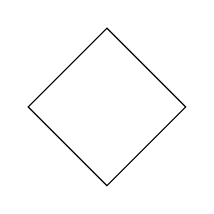
\begin{tikzpicture} 
\draw (1,0) -- (0,1) -- (-1,0) -- (0,-1) -- cycle; 
\end{tikzpicture}

\begin{tikzpicture} 
\draw[step=1,color=gray!40] (-2,-2) grid (2,2); 
\draw[->] (-3,0) -- (3,0); 
\draw[->] (0,-3) -- (0,3); 
\draw (0,0) circle (1);  
\end{tikzpicture}

\begin{tikzpicture} 
\draw[->] (-3,3) -- (3,3); 
\draw[->>] (-3,2) -- (3,2); 
\draw[->|] (-3,1) -- (3,1); 
\draw[-to] (-3,0) -- (3,0); 
\draw[-latex] (-3,-1) -- (3,-1); 
\draw[-stealth] (-3,-2) -- (3,-2); 
\end{tikzpicture}

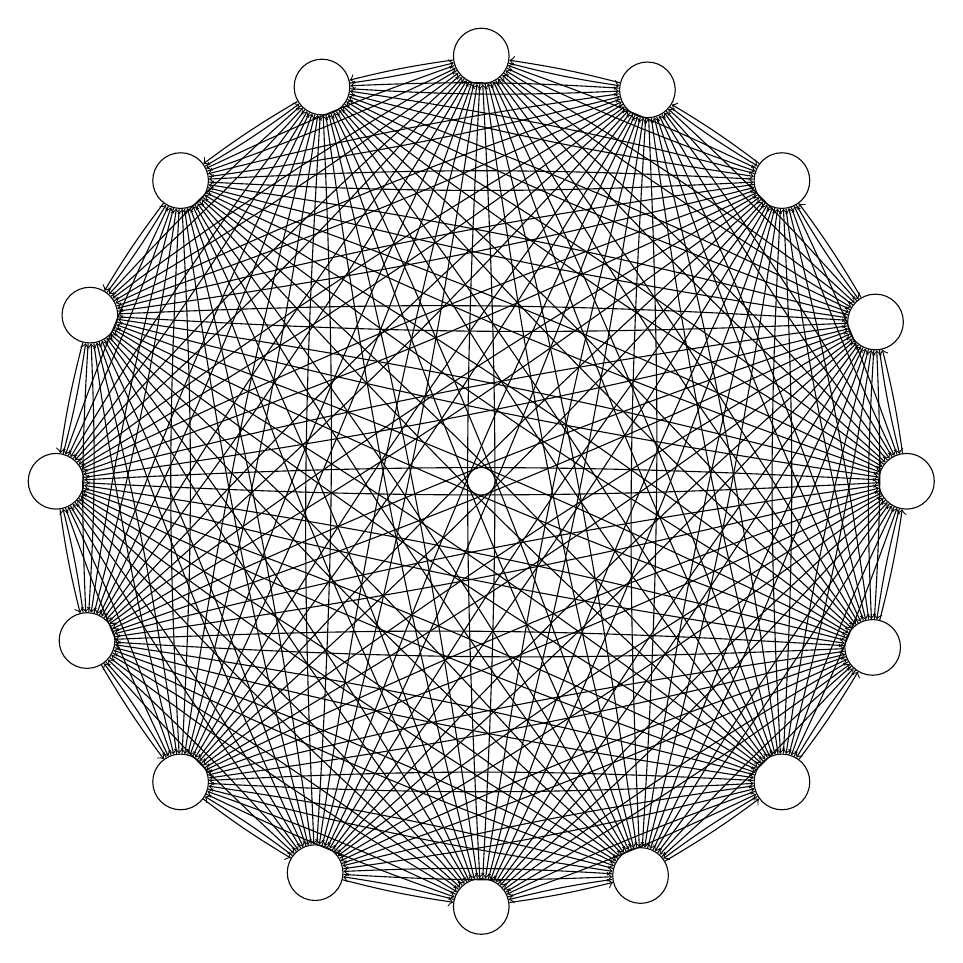
\begin{tikzpicture}[transform shape]
  %the multiplication with floats is not possible. Thus I split the loop in two.
  \foreach \number in {1,...,8}{
      % Computer angle:
        \mycount=\number
        \advance\mycount by -1
  \multiply\mycount by 45
        \advance\mycount by 0
      \node[draw,circle,inner sep=0.25cm] (N-\number) at (\the\mycount:5.4cm) {};
    }
  \foreach \number in {9,...,16}{
      % Computer angle:
        \mycount=\number
        \advance\mycount by -1
  \multiply\mycount by 45
        \advance\mycount by 22.5
      \node[draw,circle,inner sep=0.25cm] (N-\number) at (\the\mycount:5.4cm) {};
    }
  \foreach \number in {1,...,15}{
        \mycount=\number
        \advance\mycount by 1
  \foreach \numbera in {\the\mycount,...,16}{
    \path (N-\number) edge[->,bend right=3] (N-\numbera)  edge[<-,bend
      left=3] (N-\numbera);
  }
}
\end{tikzpicture}

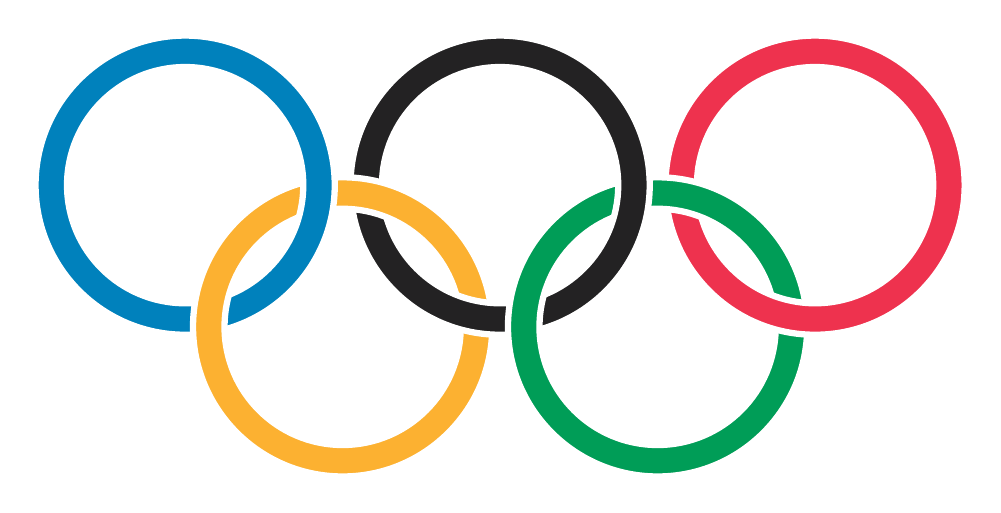
\begin{tikzpicture}
 \definecolor{r1}{RGB}{0,129,188}
 \definecolor{r2}{RGB}{252,177,49}
 \definecolor{r3}{RGB}{35,34,35}
 \definecolor{r4}{RGB}{0,157,87}
 \definecolor{r5}{RGB}{238,50,78}
 \begin{scope}
   \clip (-6,2) rectangle (6,-.9);
   \foreach \col/\xp/\yp in {
     r5/4/0, r4/2/-1.8, r3/0/0,
     r2/-2/-1.8, r1/-4/0
   } {
     \path[draw=white,line width=.08cm,
     fill=\col,even odd rule]
     (\xp, \yp) circle (1.9cm)
     (\xp, \yp) circle (1.5cm);
   }
 \end{scope}
 \begin{scope}
   \clip (-6,-.9) rectangle (6,-3.8);
   \foreach \col/\xp/\yp in {
     r1/-4/0, r2/-2/-1.8, r3/0/0,
     r4/2/-1.8, r5/4/0
   } {
     \path[draw=white,line width=.08cm,
     fill=\col,even odd rule]
     (\xp, \yp) circle (1.9cm)
     (\xp, \yp) circle (1.5cm);
   }
 \end{scope}
\end{tikzpicture}



\begin{tikzpicture}

  %color one half of a unit circle
  \begin{scope}
    \clip (0,0) circle (1cm);
    \fill[black] (0cm,1cm) rectangle (-1cm, -1cm);
  \end{scope}

  %fill heads
  \fill[black] (0,0.5) circle (0.5cm);
  \fill[white] (0,-0.5) circle (0.5cm);

  %fill eyes
  \fill[white] (0,0.5) circle (0.1cm);
  \fill[black] (0,-0.5) circle (0.1cm);

  %outer line
  \draw (0,0) circle (1cm);

\end{tikzpicture}


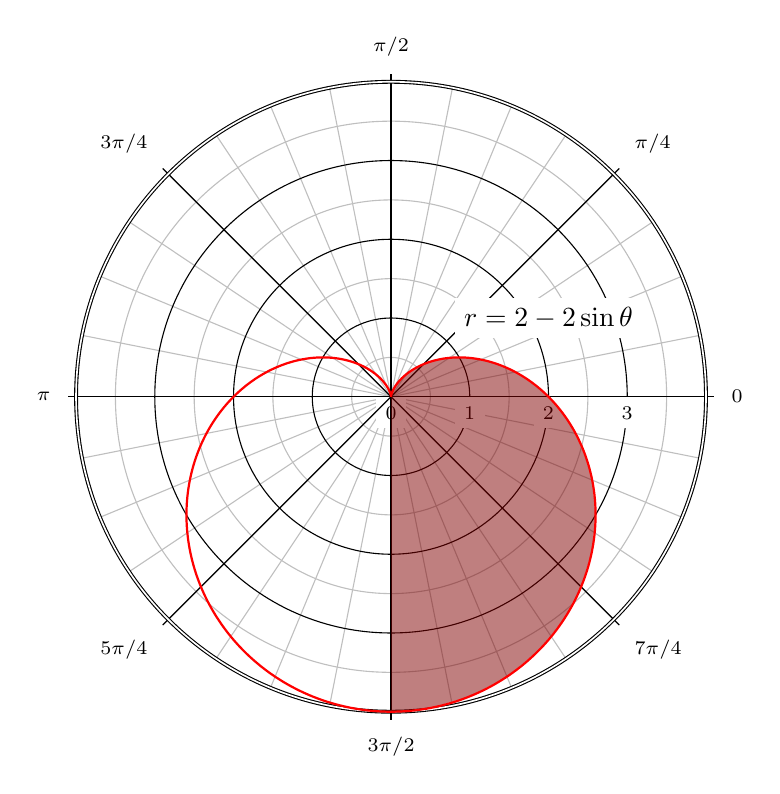
\begin{tikzpicture}[>=latex]

% Draw the lines at multiples of pi/12
\foreach \ang in {0,...,31} {
  \draw [lightgray] (0,0) -- (\ang * 180 / 16:4);
}

% Concentric circles and radius labels
\foreach \s in {0, 1, 2, 3} {
  \draw [lightgray] (0,0) circle (\s + 0.5);
  \draw (0,0) circle (\s);
  \node [fill=white] at (\s, 0) [below] {\scriptsize $\s$};
}

% Add the labels at multiples of pi/4
\foreach \ang/\lab/\dir in {
  0/0/right,
  1/{\pi/4}/{above right},
  2/{\pi/2}/above,
  3/{3\pi/4}/{above left},
  4/{\pi}/left,
  5/{5\pi/4}/{below left},
  7/{7\pi/4}/{below right},
  6/{3\pi/2}/below} {
  \draw (0,0) -- (\ang * 180 / 4:4.1);
  \node [fill=white] at (\ang * 180 / 4:4.2) [\dir] {\scriptsize $\lab$};
}

% The double-lined circle around the whole diagram
\draw [style=double] (0,0) circle (4);

\fill [fill=red!50!black, opacity=0.5] plot [domain=-pi/2:pi/2]
  (xy polar cs:angle=\x r, radius= {2-2*sin(\x r)});
\draw [thick, color=red, domain=0:2*pi, samples=200, smooth]
  plot (xy polar cs:angle=\x r, radius={2-2*sin(\x r)});
\node [fill=white] at (2,1) {$r=2-2\sin\theta$};

\end{tikzpicture} 


% definition de partial ellipse
\tikzset{partial ellipse/.style args =
  {#1:#2:#3}{insert path={+ (#1:#3) arc (#1:#2:#3)}}}
\begin{tikzpicture}[>=latex]
  %  ellipses
  \draw [fill=white!90!red]    (3,-1.8) ellipse    (4cm and 1 cm);
  \draw [fill=yellow!90!green] (3,-1.8) ellipse (3cm and 0.75 cm);
  \draw [fill=white!90!green]  (3,-1.8) ellipse  (2cm and 0.5 cm);

  % -- Soleil
  \shade [ball color=gray!10!yellow] (3,-1.8) circle (1);
  \node (soleil) at (3,-1.8) {\bf Soleil};
  % partial ellipse pour tracé devant le Soleil
  \draw (3,-1.8) [partial ellipse=220:320:2cm and 0.5cm]
        (3,-1.8) [partial ellipse=220:320:3cm and 0.75cm];

  % Venus
  \shade [ball color=gray!10!orange] (1.6,-1.8) circle (.2);
  \node (venus) at (1.5,-1.45) {Venus}; 

  % ombre de Venus
  \draw[color=white!70!black,fill=white!70!black]
    (1.6,-2.3) ellipse (2mm and 0.5mm);

  % Mercure
  \shade [ball color=gray!10!orange] (5,-1.225) circle (.25);
  \node (mercure) at (5,-0.8) {Mercure}; 

  % Earth
  \shade [ball color=white!50!blue] (5.75,-2.5) circle (.33);
  \node (terre) at (6.6,-2.6) {\bf Terre};

  % Lune
  \shade [ball color=yellow] (5.25,-2.8) circle (.1);
  \node (lune) at (5.25,-3) {Lune};
     
  % Mars
  \draw (3,-1.8) [partial ellipse=45:120:9cm and 2.5cm];
  \shade [ball color=black!50!red] (5,0.66) circle (.15);
  \node (mars) at (5,1) {\bf Mars};   
  % trajet
  \draw [line width=2pt,blue,->,>=latex] (terre) to[out=0,in=0] (mars);   
\end{tikzpicture}

\end{center}

\end{document}
